% -----------------------------------------------------------------------------
% ########################
% # PREDLOGA ZA POROCILO #
% ########################
%
% @author Tilen Miklavič, Luka Zornada, Rihard Marušič
% @date   20. december 2020
%
\documentclass[a4paper,12pt]{report}

% -----------------------------------------------------------------------------
% ####################################################
% # UPORABA PAKETOV - NASTAVITEV JEZIKA in KODIRANJA #
% ####################################################
\usepackage[slovene]{babel}
\usepackage[utf8]{inputenc}
\usepackage{lmodern}
\usepackage[T1]{fontenc}
\usepackage[sc]{mathpazo}
\linespread{1.05}
\usepackage[T1]{fontenc}

% -----------------------------------------------------------------------------
% ######################################
% # VNOS KLJUCNIH PARAMETROV BESEDILA  #
% ######################################

\newcommand{\naslov}     {Spletna knjigarna - Trgovina abc}
\newcommand{\prviavtor}  {Tilen Miklavič}
\newcommand{\prviindeks} {63180204}
\newcommand{\drugiavtor} {Jana Novak}
\newcommand{\drugiindeks}{63000001}
\newcommand{\tretjiavtor} {Marija Novak}
\newcommand{\tretjiindeks}{63000002}
\newcommand{\kraj}       {Ljubljana}

% -----------------------------------------------------------------------------
% ###################
% # UPORABA PAKETOV #
% ###################
\usepackage[a4paper,left=25mm,right=25mm,top=20mm,bottom=30mm,includehead]{geometry}

\usepackage{graphicx, epsfig}

\usepackage{fancyhdr}

\usepackage[
colorlinks=true, linkcolor=blue, citecolor=red,
%
pdftitle={\naslov},
pdfauthor={\prviavtor, \drugiavtor},
pdfsubject={Poročilo seminarske naloge pri predmetu Elektronsko Poslovanje},
pdfkeywords={spletna prodajalna, PHP, SSL, MySQL}, a4paper, pagebackref=true, unicode]{hyperref}

% -----------------------------------------------------------------------------
\begin{document}

% -----------------------------------------------------------------------------
% ##################
% # NASLOVNA STRAN #
% ##################
\begin{titlepage}
	\begin{center}
	{UNIVERZA V LJUBLJANI\\[10pt] 
	FAKULTETA ZA RAČUNALNIŠTVO IN INFORMATIKO}

	\vspace{65mm}

	{\Large\textbf{\naslov}}

	\vspace{10mm}

	{\large Poročilo seminarske naloge pri predmetu\\[10pt] Elektronsko poslovanje}

	\vfill
	\vspace{60mm}

\hspace{20mm}
\begin{minipage}[t]{70mm}
	{\bf Študenti}\\
	{\prviavtor} ({\prviindeks})\\ 
	{\drugiavtor} ({\drugiindeks})\\
	{\tretjiavtor} ({\tretjiindeks})
\end{minipage}
%\hfill
\begin{minipage}[t]{50mm}
	{\bf Mentor}\\
	David Jelenc
\end{minipage}
%\hspace{20mm}

	\vspace{35mm}

	{	\kraj, \today}
	\end{center}
\end{titlepage}

% -----------------------------------------------------------------------------
% ##################
% # KAZALO VSEBINE #
% ##################

\tableofcontents

% -----------------------------------------------------------------------------
% ############
% # POVZETEK #
% ############
%\begin{abstract}
%\end{abstract}

% -----------------------------------------------------------------------------
% ##################
% # UVOD DOKUMENTA #
% ##################
\chapter{Uvod}

Za seminarsko nalogo smo izdelali spletno knjigarno. Namenjena je anonimnim in registriranim kupcem, ter jim ogomoča pregled artiklov in dodajanje le teh v košarico. Ravno tako podpira prijavo in registracijo novih uporabnikov. Spletno knjigarno ravno tako uporabljajo prodajalci, ki imajo pregled nad strankami in lahko z njihovimi podatki upravljajo. Njihova naloga pa je tudi potrjevanje, zavračanje in storniranje računov. Za sistem skrbi sistemski inženir (admin), ki ima pregled nad vsemi trgovci. 

% -----------------------------------------------
\chapter{Navedba realiziranih storitev}

Implementirali smo reigstracijo strank z uporabo filtriranja CAPTCHA. Za to smo uporabili Googlovo reCAPTCHA, ki se na strani za registracijo pojavi kot enostaven gumb za potrditev, da uporabnik ni robot. \newline 

Implementirali smo tudi registracijo strank z uporabo potrditvenega e-maila. Za to smo uporabili priljubljeno knjižnico PHPMailer. Ob reigstraciji novega uporabnika, se le temu na vpisan e-poštni naslov pošlje sporočilo z vsemi podatki, ravno tako pa povezava do strani za potrditev e-poštnega naslova. Preden uporabnik potrdi svoj e-mail, je v bazi označen kot neaktiven, ko pa obišče povezavo za potrditev, se spremeni v "aktivnega" kupca. \newline

Implementirali smo smiselno organizacijo in izvedbo uporabniškega vmesnika s pomočjo tehnologij kot so sta CSS in JavaScript. Za to smo uporabili CSS in JS knjižnico Bootstrap, ki nam v večini koristi za smiselen celoten estetski izgled strani. 

Implementirali smo binarno iskanje... \newline

Predstavitev artiklov s slikami... \newline

Implementirali smo ocenjevanje artiklov. Do te funkcionalnosti lahko dostopajo samo prijavljeni uporabniki, ko kliknejo na artikel, da se jim pokažejo podrobnosti. Na tej strani lahko podajo svojo oceno za določen artikel, ta pa se nato shrani v podatkovno bazo. Na strani s pregledom artiklov lahko vsak vidi povprečno oceno posamičnega artikla. \newline



Obvezne storitve, ki je nismo implementirali do konca je Prikaz artiklov v mobilni aplikaciji Android. Razvili smo REST API-je za pregled, urejanje in brisanje artiklov, vendar je bil JSON element, ki ga je Android aplikacija prejemala pokvarjen in ga zato nu mogla pretvoriti v Kotlin objekt. 


% -----------------------------------------------
\chapter{Podatkovni model}

\begin{figure}[htp]
    \centering
    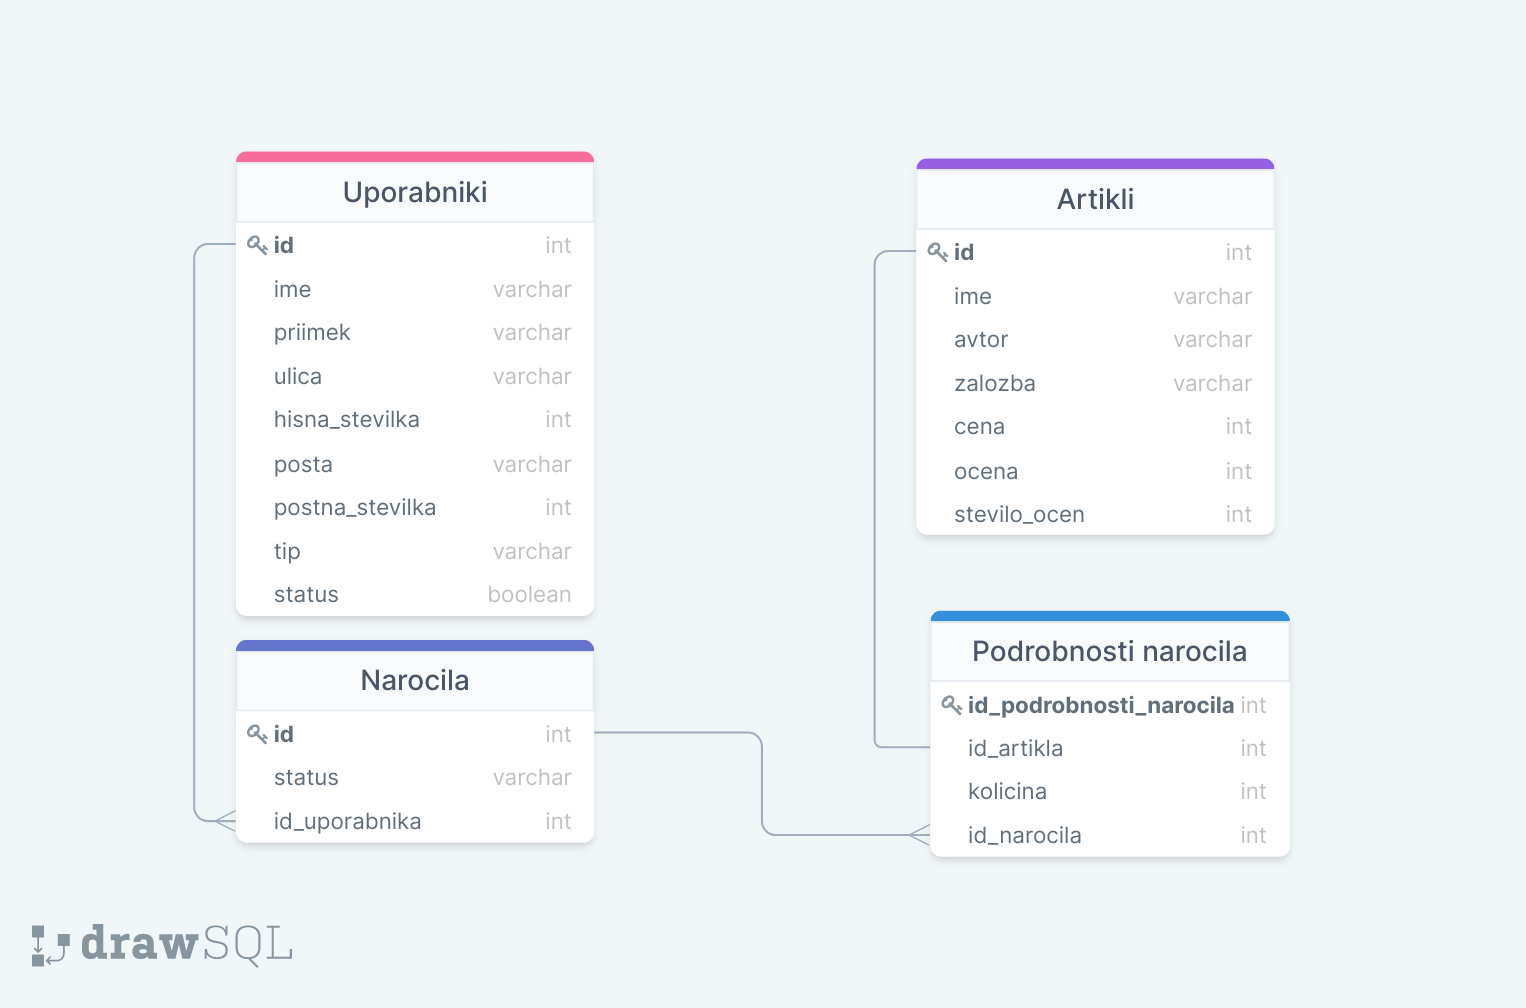
\includegraphics[width=15cm]{img/sql.png}
    \caption{Podatkovni model}
    \label{fig:galaxy}
\end{figure}

S podatkovnega modela je razvidno, da smo ustvarili štiri tabele (artikli, uporabniki, narocila, podrobnosti narocila). V tabeli artikli so shranjeni seveda vsi artikli ki se prodajajo v knjigarni, v tabeli uporabniki si shranjeni vsi uporabniki spletne trgovine (admin, prodajalci in stranke), v tabeli narocila so shranjena vsa narocila in v tabeli podrobnosti narocila so shranjeni vsi artikli ki so se pojavili na kakšnem naročilu (vsak zapis v podrobnosti naročila ponazarja eno naročilo in en artikel, ki je na tem naročilu, ravno tako pa nam pove količino tega izdelka na tem določenim naročilom).


% -----------------------------------------------
\chapter{Varnost sistema}

Varnostni kanali... \newline

Prijava v spletno trgovino je zaščitena z uporabniškim imenom in geslom. Ravno tako je prijava v sistem kot prodajalec ali administrator zaščitena s certifikatom. \newline

Vsa gesla se pred vpisom v podatkovno bazo šifrira in se jih nato vedno preverja v funkvciji v šifrirani obliki.  \newline

S funkcijo htmlspecialchard() je naša spletna knjigarna zaščitena pred napadi XSS. \newline

Z uporabo PDO-ja pa je zaščitena tudi pred SQL-injection napadi. \newline


% -----------------------------------------------
\chapter{Izjava o avtorstvu seminarske naloge}

Spodaj podpisani \textit{\prviavtor}, vpisna številka \textit{\prviindeks}, sem (so)avtor seminarske naloge z naslovom \textit{\naslov}. S svojim podpisom zagotavljam, da sem izdelal ali bil soudeležen pri izdelavi naslednjih sklopov seminarske naloge:
\begin{itemize}
    \item Zasnova MySQL podatkovnega modela 
	\item Kreiranje MySQL podatkovnega modela
	\item Kreiranje vseh tabel v bazi
	\item Vzpostavljanje lastne certifikatne agencije 
	\item Izdelovanje strežniškega digitalnega potrdila
	\item Implementacija večinskega dela index.php routerja
	\item Implementacija večinskega dela database.php datotek za komunikacijo s podatkovno bazo 
	\item Implementacija logike za Prikaz seznama artiklov prijavljeni in neprijavljeni stranki 
	\item Implementacija logike za prikaz podrobnosti artikla prijavljeni in neprijavljeni stranki 
	\item Implementacija logike za prijavo in registracijo stranke 
	\item Implementacija logike za dodajanje artiklov v košarico 
	\item Posodabljanje lastnih atributov vseh uporabnikov 
	\item Posodabljanje atributov drugim uporabnikom 
	\item Ocenjevanja artiklov 
	\item Šifriranje gesel 
	\item Obramba pred napadi XSS
	\item Obmramba pred napadi SQL injection 
	\item Kreiranje novega artikla za prodajalca
	\item Urejanje artiklov za prodajalca 
	\item Pregled strank za prodajalca 
	\item Urejanje atributov strank za prodajalca
	\item Ustvarjanje novih uporabnikov za prodajalca
	\item Pregled in urejanje prodajalcev za admina 
	\item Ustvarjanje novih prodajalcev za admina
	\item Shranjevanje trenutne seje za ohranitev prijave in brisanje seje ob odjavi 
	\item Implementiranje filtriranja ob registraciji z CAPTCHA
	\item Implementiranje potrjevanja strank s potrditvenim emailom
	\item Implementacija API endpoint-a
	\item Implementacija kontrolerja za komuniciranje med strežnikom in android apikacijo 
	\item priprava izgleda in delovanje android aplikacije (nepopolno)
	
\end{itemize}

Podpis: {\prviavtor}, l.r.

\newpage

Spodaj podpisana \textit{\drugiavtor}, vpisna številka \textit{\drugiindeks}, sem (so)avtor seminarske naloge z naslovom \textit{\naslov}. S svojim podpisom zagotavljam, da sem izdelal ali bil soudeležen pri izdelavi naslednjih sklopov seminarske naloge:
\begin{itemize}
    \item Vzorčni sklop 1
	 \item Vzorčni sklop 2
\end{itemize}

Podpis: {\drugiavtor}, l.r.

\newpage

Spodaj podpisana \textit{\tretjiavtor}, vpisna številka \textit{\tretjiindeks}, sem (so)avtor seminarske naloge z naslovom \textit{\naslov}. S svojim podpisom zagotavljam, da sem izdelal ali bil soudeležen pri izdelavi naslednjih sklopov seminarske naloge:
\begin{itemize}
    \item Vzorčni sklop 1
	 \item Vzorčni sklop 2
\end{itemize}

Podpis: {\tretjiavtor}, l.r.








\end{document}
